\documentclass{beamer}
\usepackage[utf8]{inputenc}


\usetheme{Madrid}
\usecolortheme{default}
\useinnertheme{circles}
\usepackage{tikz}
\setbeamercovered{dynamic}

\definecolor{Logo1}{rgb}{0.208, 0.2865, 0.373}
\definecolor{Logo2}{rgb}{0.000, 0.674, 0.863}

\setbeamercolor*{palette primary}{bg=Logo1, fg=white}
\setbeamercolor*{palette secondary}{bg=Logo2, fg=white}
\setbeamercolor*{palette tertiary}{bg=white, fg=Logo1}
\setbeamercolor*{palette quaternary}{bg=Logo1,fg=white}
\setbeamercolor{structure}{fg=Logo1} % itemize, enumerate, etc
\setbeamercolor{section in toc}{fg=Logo1} % TOC sections

%------------------------------------------------------------
%This block of code defines the information to appear in the
%Title page
\title{Реалізація кубитів для квантових комп'ютерів.}

%\subtitle{And its subtitle}

\author{Мнацаканов Антон}

\institute[КПІ] % (optional)
{
  Національний технічний університет України\\
  "Київський політехнічний інститут імені Ігоря Сікорського"
}

\date{\today}


%\logo{\includegraphics[height=.5cm]{logo-footer.png}}

%End of title page configuration block
%------------------------------------------------------------



%------------------------------------------------------------
%The next block of commands puts the table of contents at the 
%beginning of each section and highlights the current section:

\AtBeginSection[]
{
  \begin{frame}
    \frametitle{Зміст}
    \tableofcontents[currentsection]
  \end{frame}
}
%------------------------------------------------------------
\usepackage{array}
\usepackage{colortbl}
\usepackage{hhline}
\usepackage[english,ukrainian,russian]{babel}
%\usepackage{fourier}
\usepackage{lmodern}


\usepackage{ textcomp }
\usepackage{ eqnarray }
\usepackage{ txfonts }
\usepackage{hyperref}

\begin{document}

%The next statement creates the title page.
\frame{\titlepage}


%---------------------------------------------------------
%This block of code is for the table of contents after
%the title page
\begin{frame}
\frametitle{Зміст}
\tableofcontents
\end{frame}
%---------------------------------------------------------


\section{Визначення}

%---------------------------------------------------------
%Changing visivility of the text
{\title{Що таке кубіт?}
\usebackgroundtemplate{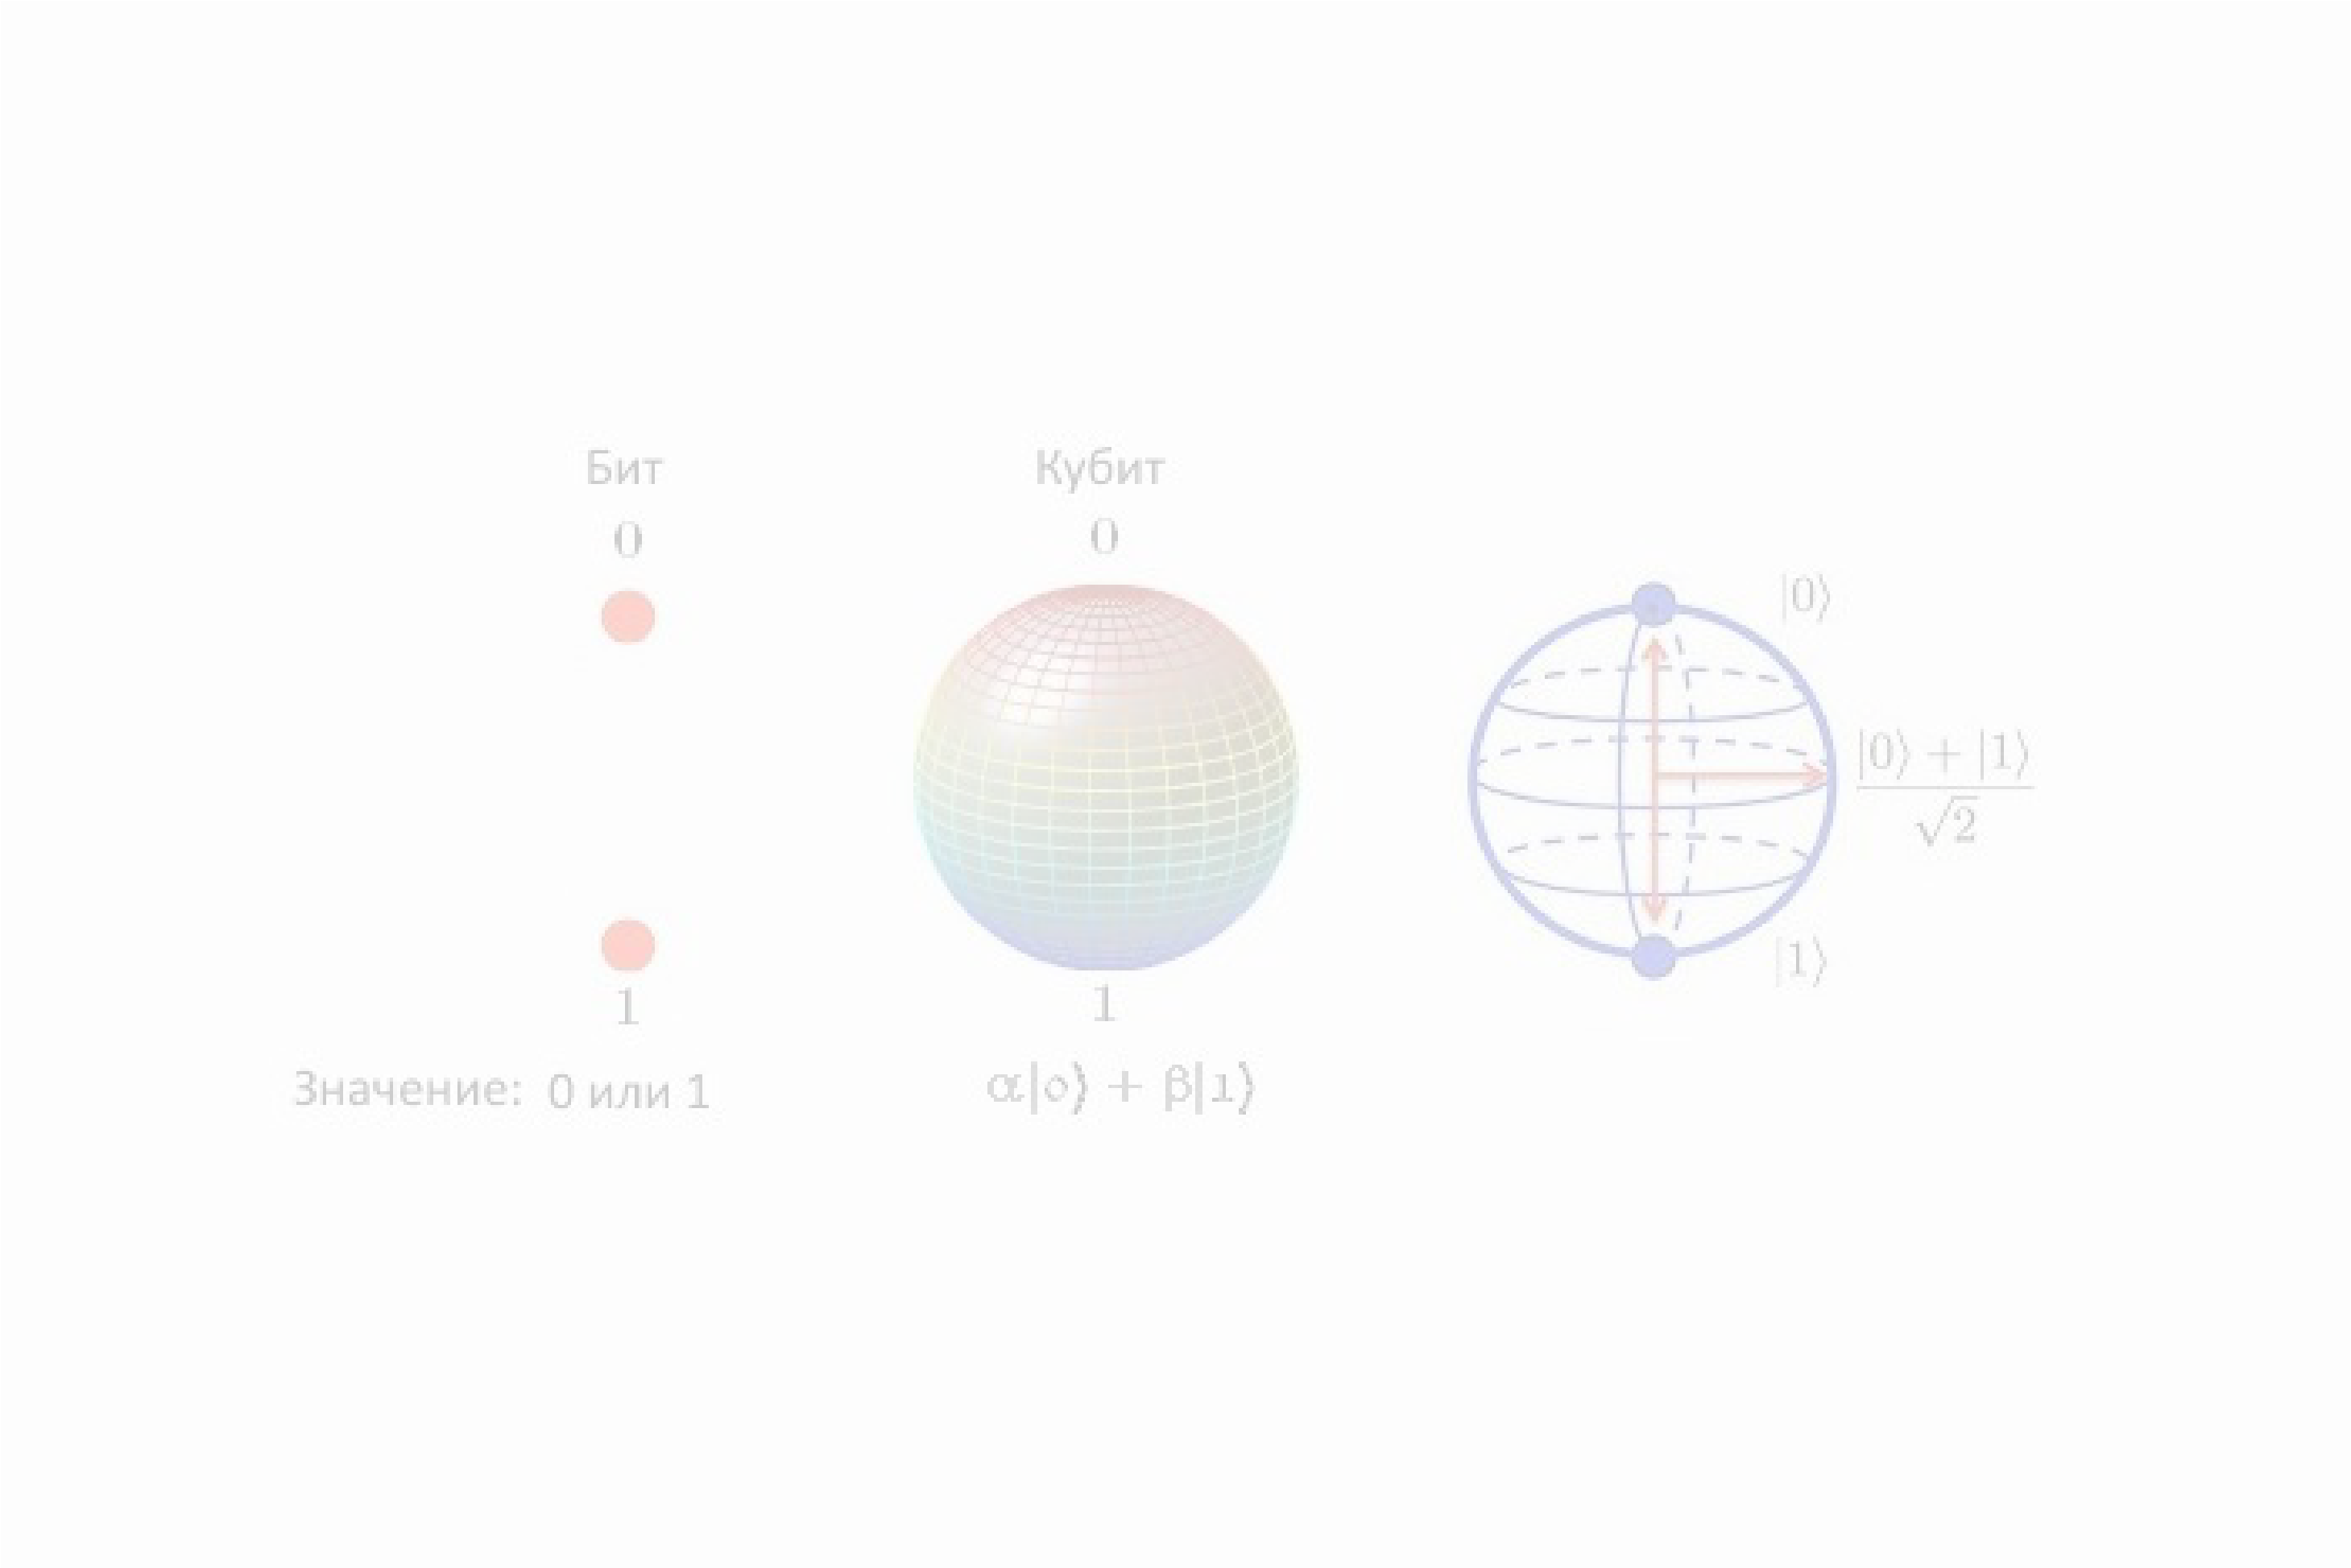
\includegraphics[width=\paperwidth]{1.png}}
\begin{frame}
\frametitle{Що таке кубіт?}
 Кубіт — це дворівнева квантовомеханічна система, наприклад, поляризація окремого фотона, яка може бути вертикальною або горизонтальною. В класичній системі біт завжди прийматиме одне з двох значень, але квантова механіка дозволяє кубітові перебувати в стані суперпозиції. Ця властивість кубіта є базисом для всієї теорії квантових обчислень.
\end{frame}
}
%---------------------------------------------------------
\section{Порівняння}

%---------------------------------------------------------
%Example of the \pause command
\title{Порівняння кубітів та бітів}
\usebackgroundtemplate{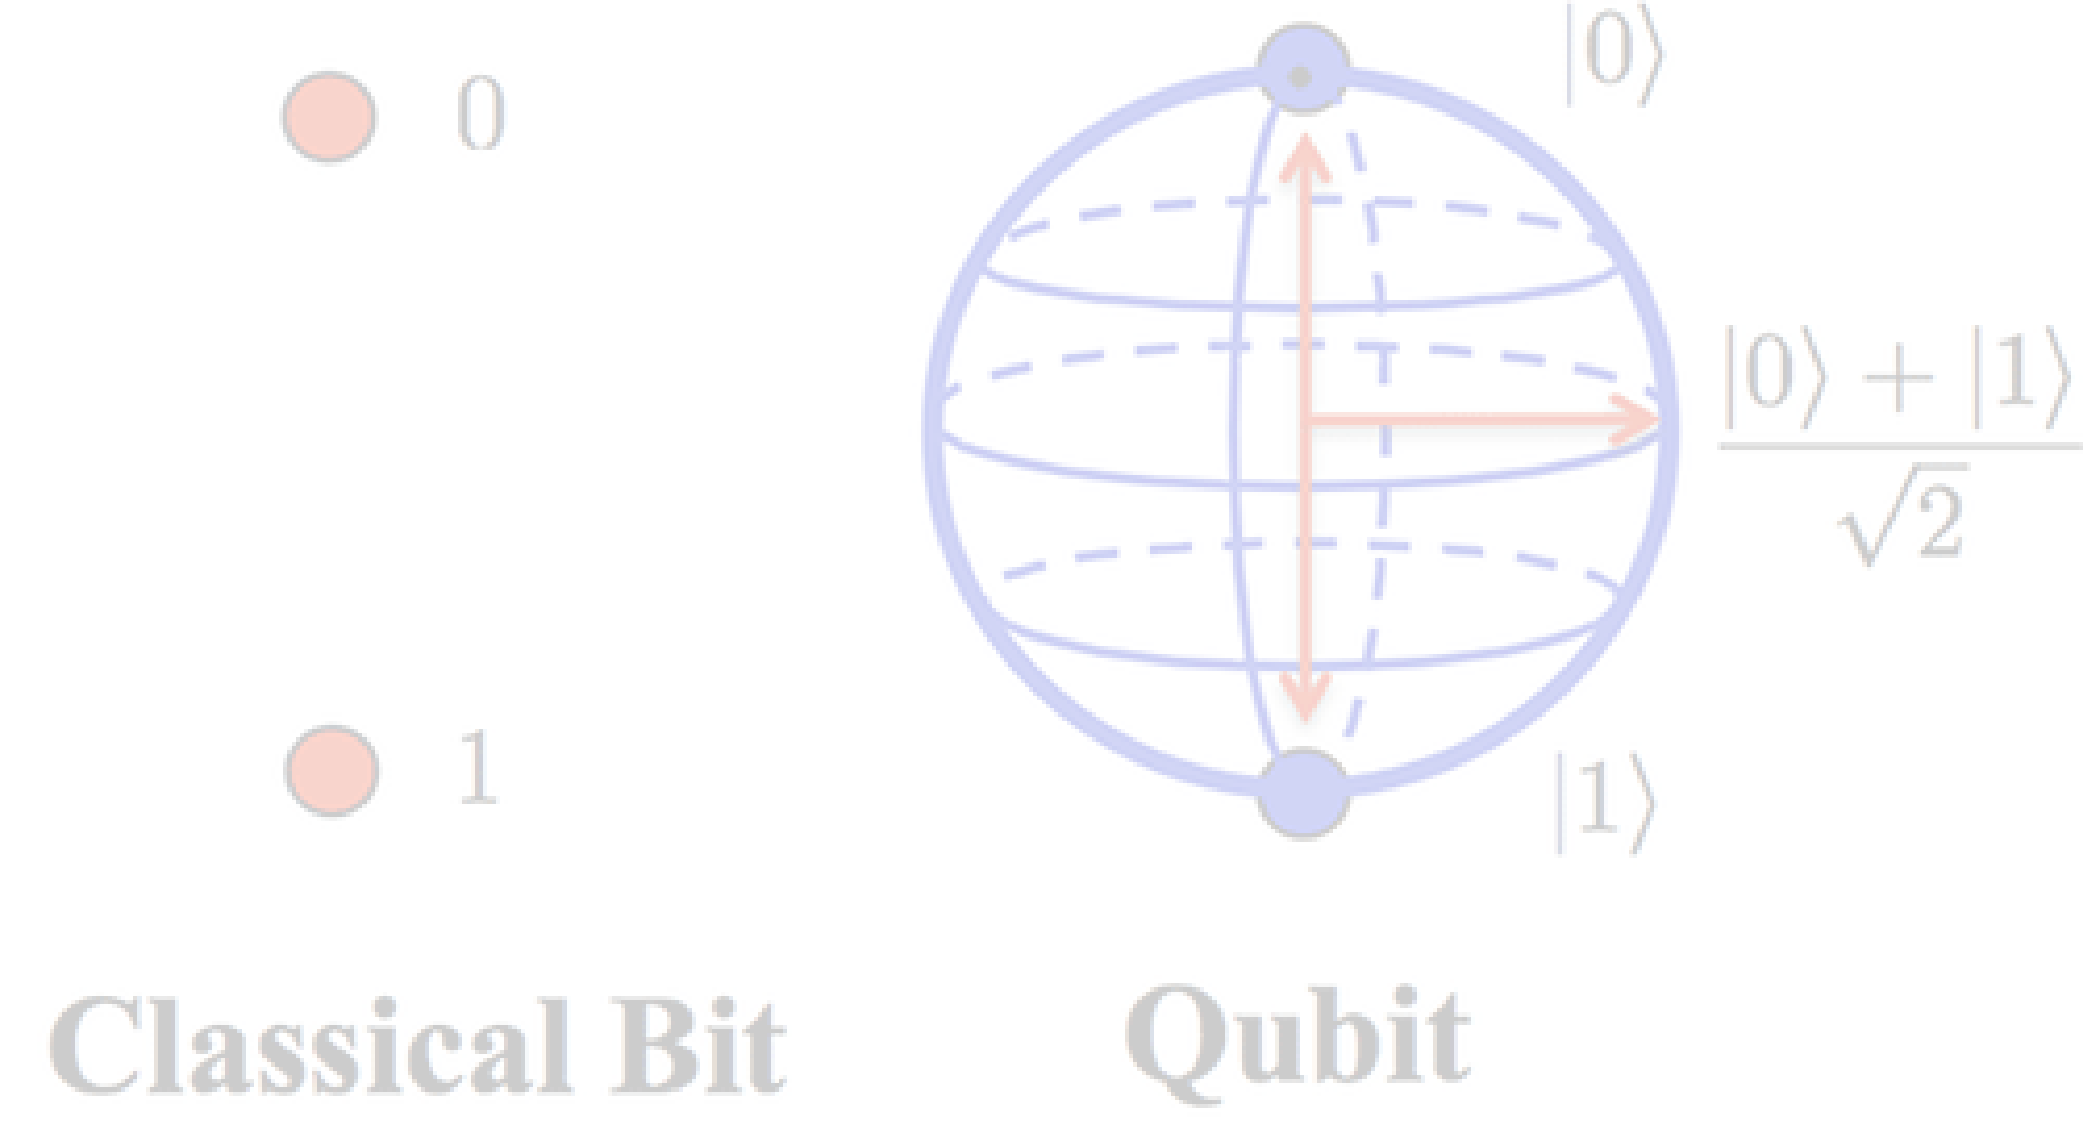
\includegraphics[height=0.5\textwidth]{2.png}}
\begin{frame}
\frametitle{Pізниця біта і  кубітa}
Кубіти представлені суперпозицією безлічі можливих станів
Для досягнення лінійного поєднання двох станів кубіт використовує явище квантової механіки, яке називається суперпозицією. Класичний двійковий біт може становити лише одне двійкове значення, наприклад 0 або 1. Це означає, що біт може перебувати тільки в одному з двох можливих станів. Кубит може представляти 0, 1 або будь-яку частку від 0 до 1 в суперпозиції обох станів з певною ймовірністю того, що він дорівнює 0, і певною ймовірністю того, що він дорівнює 1.
\end{frame}
%---------------------------------------------------------
\usebackgroundtemplate{}
\begin{frame}
\frametitle{Pізниця біта і  кубітa}
У той час як для повного опису системи з n класичних бітів достатньо n нулів і одиниць, для опису системи з кубитів n необхідно (2n - 1) комплексних чисел. Це з тим, що n-кубитную систему можна представить як вектор у 2n-мірному \href{https://en.wikipedia.org/wiki/Hilbert_space}{Гільбертовом просторі}. Звідси випливає, що система з кубітів може вмістити експоненційно більше інформації, ніж система з бітів.
\center{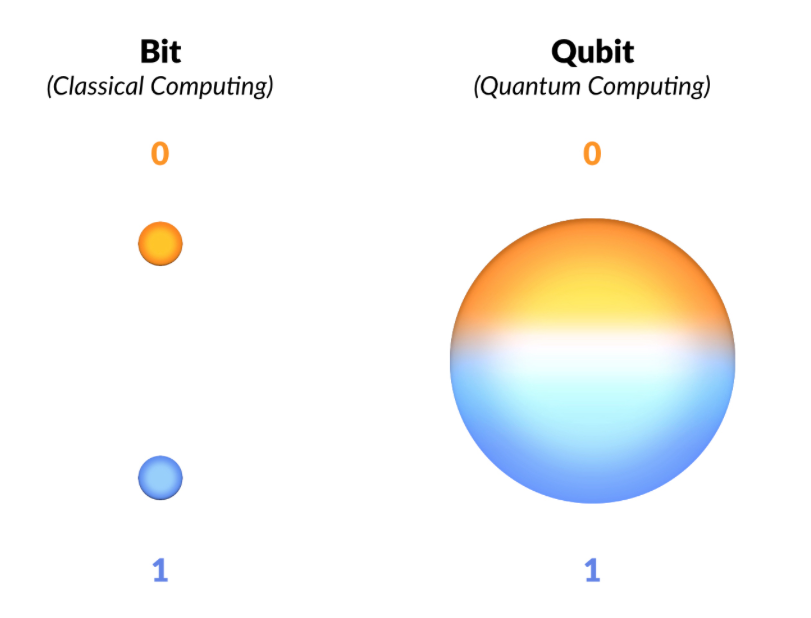
\includegraphics[width=0.5\linewidth]{3.png}}

\end{frame}


%---------------------------------------------------------
%Highlighting text
\title{Стан кубіту}
\usebackgroundtemplate{}
\begin{frame}
\frametitle{Стан кубіту}
Як і біт, кубіт допускає два власні стани, що позначаються  |0$\rangle$ і   |1$\rangle$ (позначення Дірака), але при цьому може знаходитися і в їх суперпозиції. У загальному випадку його хвильова функція має вигляд    A|0$\rangle$ +B|1$\rangle$, де  A і B називаються амплітудами ймовірностей і є комплексними числами, що задовольняють умові   $|A|^{2}+|B|^{2}= 1$. Стан кубіту зручно представляти як стрілку на сфері Блоха.\\ 
\center{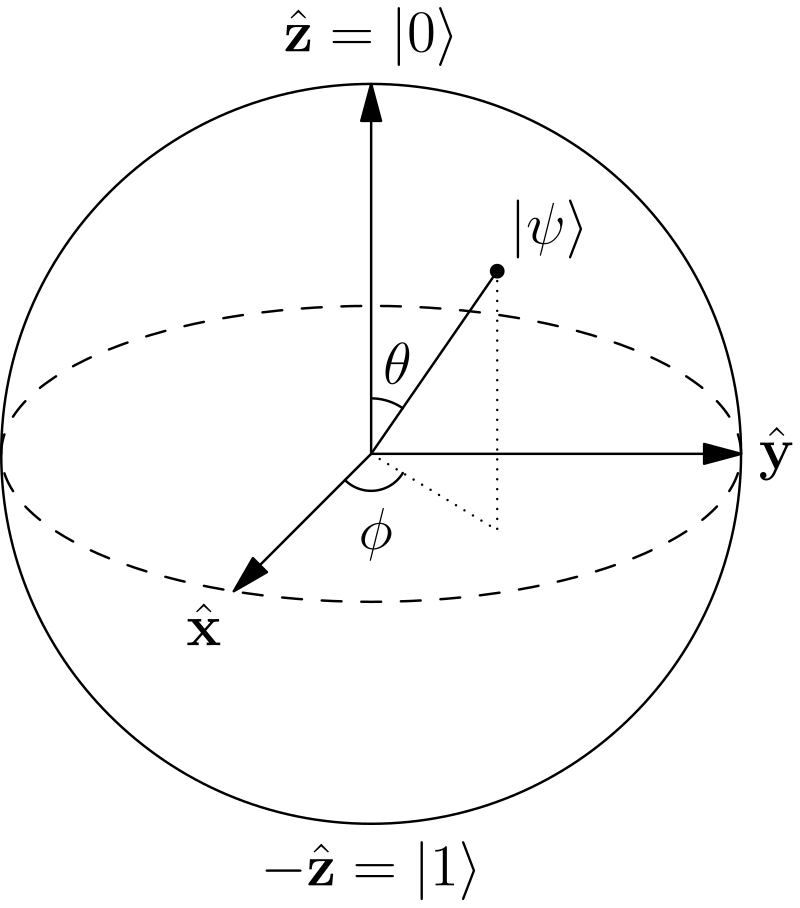
\includegraphics[width=0.3\linewidth]{4.png}}


\end{frame}
\section{Надпровідні кубити}
%---------------------------------------------------------
\usebackgroundtemplate{}
\begin{frame}
\frametitle{Надпровідні кубити}
Надпровідні кубити - це саме ті кубити, на яких працює більша частина комерційно доступних квантових процесорів. Компанія Google і IBM зробили основну ставку саме на цю технологію, оскільки такі кубити можна робити як електричні схеми, практично на друкованій платі, тільки з надпровідних матеріалів. Отримані процесори охолоджуються до низьких температур так, що метал, з якого вони виготовлені (це, як правило, алюміній), переходить у стан надпровідності. 
\center{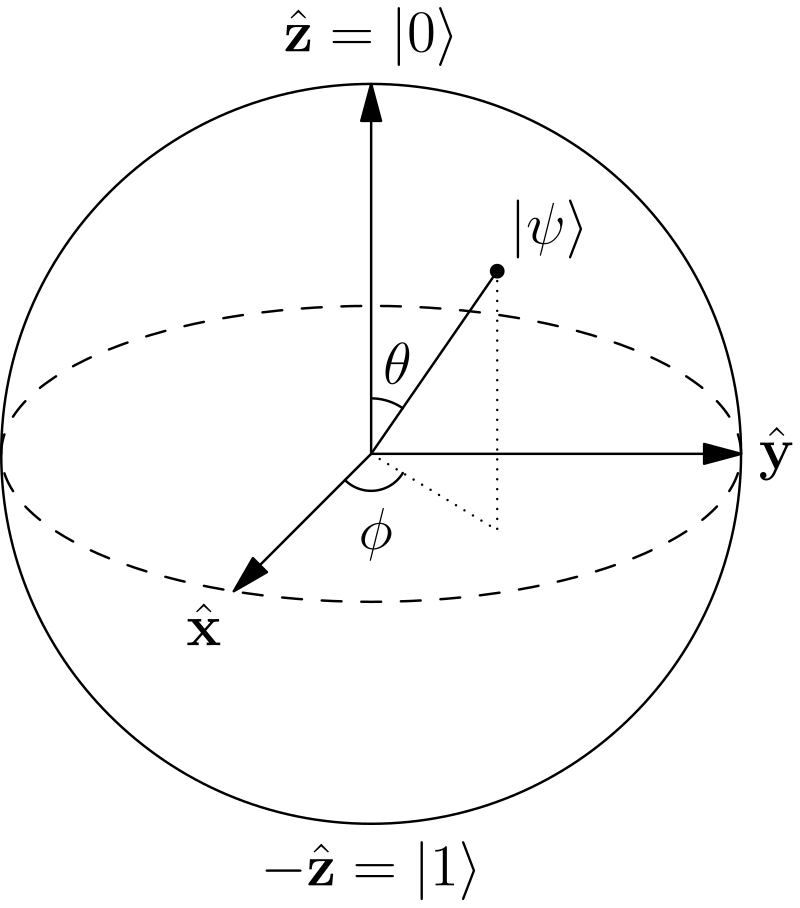
\includegraphics[width=0.3\linewidth]{4.png}}


\end{frame}



%---------------------------------------------------------
\section{Ion Trap}
%---------------------------------------------------------
\usebackgroundtemplate{}
\begin{frame}
\frametitle{Квантові комп’ютери з іонною пасткою}
... Головною особливістю комп'ютерів Ion Trap є їх стабільність; кубіти мають набагато довший «час когерентності», ніж ті, що використовуються в надпровідних квантових комп’ютерах. Незважаючи на те, що комп’ютер із іонною пасткою може працювати при кімнатній температурі, для досягнення найкращої продуктивності іони потрібно охолоджувати, але не в тій мірі, в якій цього вимагає надпровідний квантовий комп’ютер. Зв'язки між кубітами іонної пастки можна переналаштувати, тобто кожен кубіт може взаємодіяти один з одним кубітом в комп'ютері, уникаючи деяких обчислювальних витрат, які виникають із надпровідними мікросхемами.
\end{frame}




%---------------------------------------------------------

%---------------------------------------------------------
\usebackgroundtemplate{}
\begin{frame}
\frametitle{Нейтральні атоми}
Нейтральні атоми – подібний підхід до іонних пасток, але замість використання іонізованих атомів і використання їх заряду для утримання кубітів на місці використовуються нейтральні атоми та лазерний пінцет.\\ 

Нейтральні атоми мають такий самий тривалий час когерентності, що й іони (використовуються в квантових комп’ютерах із іонною пасткою). Його унікальною особливістю в порівнянні з іонними пастками є його потенціал для створення багатовимірних масивів.
\end{frame}


\usebackgroundtemplate{}
\begin{frame}
\frametitle{}
\begin{center}
Дякую за увагу!
\end{center}
\end{frame}














\end{document}